% Digital Logic Report Template
% Created: 2020-01-10, John Miller

%==========================================================
%=========== Document Setup  ==============================

% Formatting defined by class file
\documentclass[11pt]{article}

% ---- Document formatting ----
\usepackage[margin=1in]{geometry}	% Narrower margins
\usepackage{booktabs}				% Nice formatting of tables
\usepackage{graphicx}				% Ability to include graphics

%\setlength\parindent{0pt}	% Do not indent first line of paragraphs 
\usepackage[parfill]{parskip}		% Line space b/w paragraphs
%	parfill option prevents last line of pgrph from being fully justified

% Parskip package adds too much space around titles, fix with this
\RequirePackage{titlesec}
\titlespacing\section{0pt}{8pt plus 4pt minus 2pt}{3pt plus 2pt minus 2pt}
\titlespacing\subsection{0pt}{4pt plus 4pt minus 2pt}{-2pt plus 2pt minus 2pt}
\titlespacing\subsubsection{0pt}{2pt plus 4pt minus 2pt}{-6pt plus 2pt minus 2pt}

% ---- Hyperlinks ----
\usepackage[colorlinks=true,urlcolor=blue]{hyperref}	% For URL's. Automatically links internal references.

% ---- Code listings ----
\usepackage{listings} 					% Nice code layout and inclusion
\usepackage[usenames,dvipsnames]{xcolor}	% Colors (needs to be defined before using colors)

% Define custom colors for listings
\definecolor{listinggray}{gray}{0.98}		% Listings background color
\definecolor{rulegray}{gray}{0.7}			% Listings rule/frame color

% Style for Verilog
\lstdefinestyle{Verilog}{
	language=Verilog,					% Verilog
	backgroundcolor=\color{listinggray},	% light gray background
	rulecolor=\color{blue}, 			% blue frame lines
	frame=tb,							% lines above & below
	linewidth=\columnwidth, 			% set line width
	basicstyle=\small\ttfamily,	% basic font style that is used for the code	
	breaklines=true, 					% allow breaking across columns/pages
	tabsize=3,							% set tab size
	commentstyle=\color{gray},	% comments in italic 
	stringstyle=\upshape,				% strings are printed in normal font
	showspaces=false,					% don't underscore spaces
}

% How to use: \Verilog[listing_options]{file}
\newcommand{\Verilog}[2][]{%
	\lstinputlisting[style=Verilog,#1]{#2}
}




%======================================================
%=========== Body  ====================================
\begin{document}

\title{ELC 2137 Lab 9: ALU}
\author{CJ Jones}

\maketitle


\section*{Summary}

This lab explores the skill of creating a clock that drives the sequential logic to do the switching for us. The name given to this technique is time-division multiplexing (TDM). Overall, this lab demonstrated how to utilize software and programmable logic to produce a hardware output.


\section*{Q\&A}

\begin{enumerate}
	
	
	\item  What are the three main “groups” of the RTL definition of sequential logic?
	
	The three main groups of the RTL definition of sequential logic are State Memory, next state, and output logic.
	
	
	\item  Copy Figure 10.3b onto your own paper (or do it electronically) and draw three boxes around the components that belong to each group. Include your annotated figure in your report.
	
	\begin{figure}[ht]\centering
		
		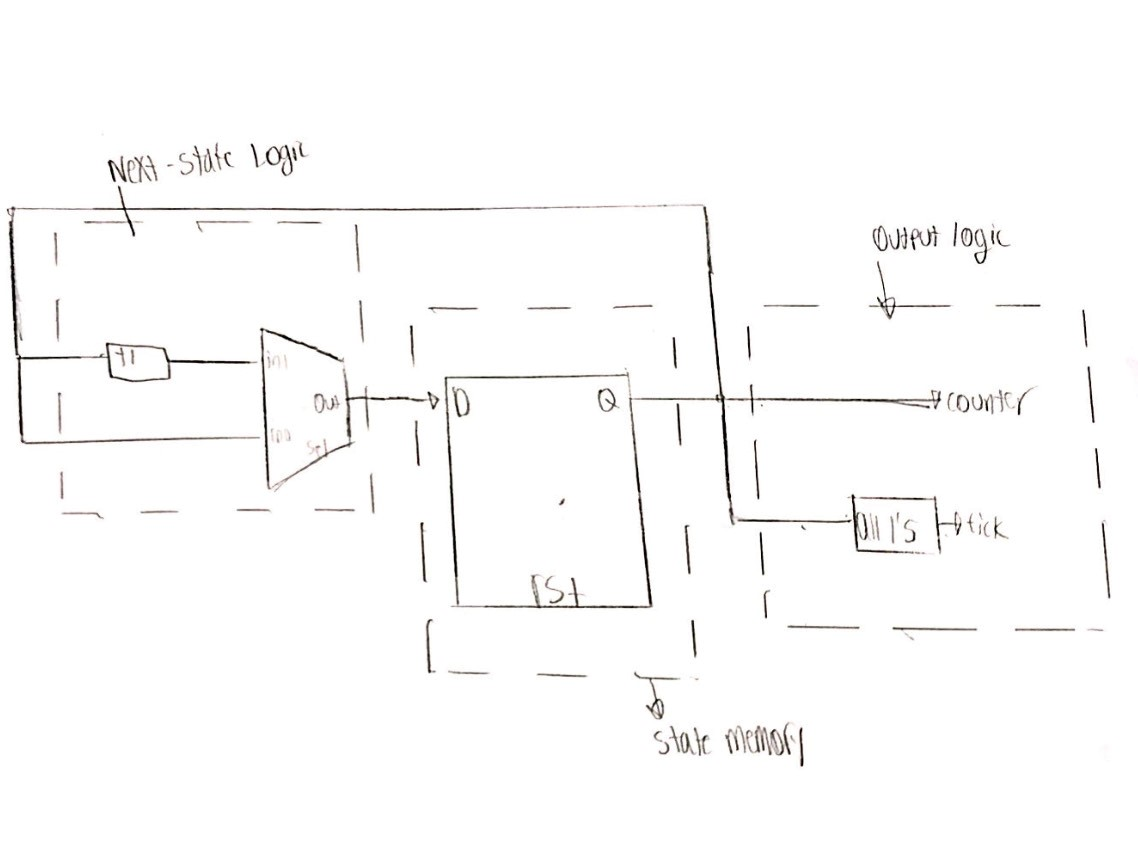
\includegraphics[width=1.0\textwidth]{10.3}
		\caption{Figure 10.3 with boxes}
		\label{fig:sim_with_table}=
	\end{figure}
\clearpage
	
	\item If instead of a counter, you wanted to make a shift register that moved the input bits from right to left (low to high). What would you put on the line Q next = /*???*/?
	
	Q next = Q reg<<1
	
\end{enumerate}











\section*{Results}


\begin{figure}[ht]\centering
	\begin{tabular}{l|rrrrrrrrrrr}
		Time (ns): & 0-5 & 5-10 & 15-20 & 20-25 & 25-30 &30-35 & 35-40 & 40-45 & 45-50 & 50-55 \\
		\midrule 
		clk& 0 &1  & 0 & 1 & 0 &1 & 0 & 1 & 0 & 1 \\
	    en& 1 &1  & 1 & 1 & 1 &1 & 1 & 1 & 1 & 1 \\
      	rst& 1 &1  & 1 & 1 & 1 &1 & 1 & 1 & 1 & 1 \\
      	count & 0 &0 & 0 & 0 & 0 &0 & 0 & 0 & 0 & 0 \\
      	tick & 0 &0  & 0 & 0 & 0 &0 & 0 & 0 & 0 & 0 \\
		
	\end{tabular}\medskip




\end{figure}
\begin{figure}[ht]\centering
	\begin{tabular}{l|rrrrrrrrrrr}
		Time (ns): & 55-60 & 60-65 & 65-70 & 70-75 & 75-80 &80-85 & 85-90 & 90-95 & 95-100 & 100-105 \\
		\midrule 
		clk& 0 &1  & 0 & 1 & 0 &1 & 0 & 1 & 0 & 1 \\
		en& 0 &0  & 0 & 0 & 0 &0 & 0 & 0 & 0 & 0 \\
		rst& 0 &0  & 0 & 0 & 0 &0 & 0 & 0 & 0 & 0 \\
		count & 0 &0 & 0 & 0 & 0 &0 & 0 & 0 & 0 & 0 \\
		tick & 0 &0  & 0 & 0 & 0 &0 & 0 & 0 & 0 & 0 \\
		
	\end{tabular}\medskip
	
	
	
	
\end{figure}
\begin{figure}[ht]\centering
	\begin{tabular}{l|rrrrrrrrrrr}
		Time (ns): & 105-110 & 110-115 & 115-120 & 120-125 & 125-130 &130-135 & 135-140 & 140-145 & 145-150 \\
		\midrule 
		clk& 1 &0  & 1 & 0 & 1 &0 & 0 & 1 & 0  \\
		en& 1 &1  & 1 & 1 & 1 &1 & 1 & 1 &1  \\
		rst& 0 &0  & 0 & 0 & 0 &0 & 0 & 0 & 0 \\ \\
		count& 1& 1 &2 & 2 & 3 & 3 &0 & 1 & 1  \\
		tick & 0 &0  & 0 & 1& 1 &0 & 0 & 0&0 \\
		
	\end{tabular}\medskip
	
	
	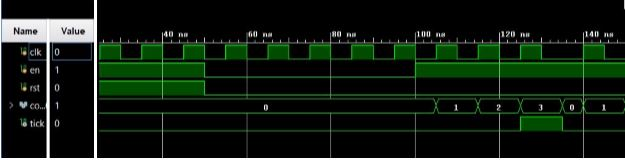
\includegraphics[width=1.0\textwidth]{Counter}
	\caption{Counterexpected results table and simulation}
	\label{fig:sim_with_table}=
	
\end{figure}

\clearpage


\begin{figure}[ht]\centering
	
	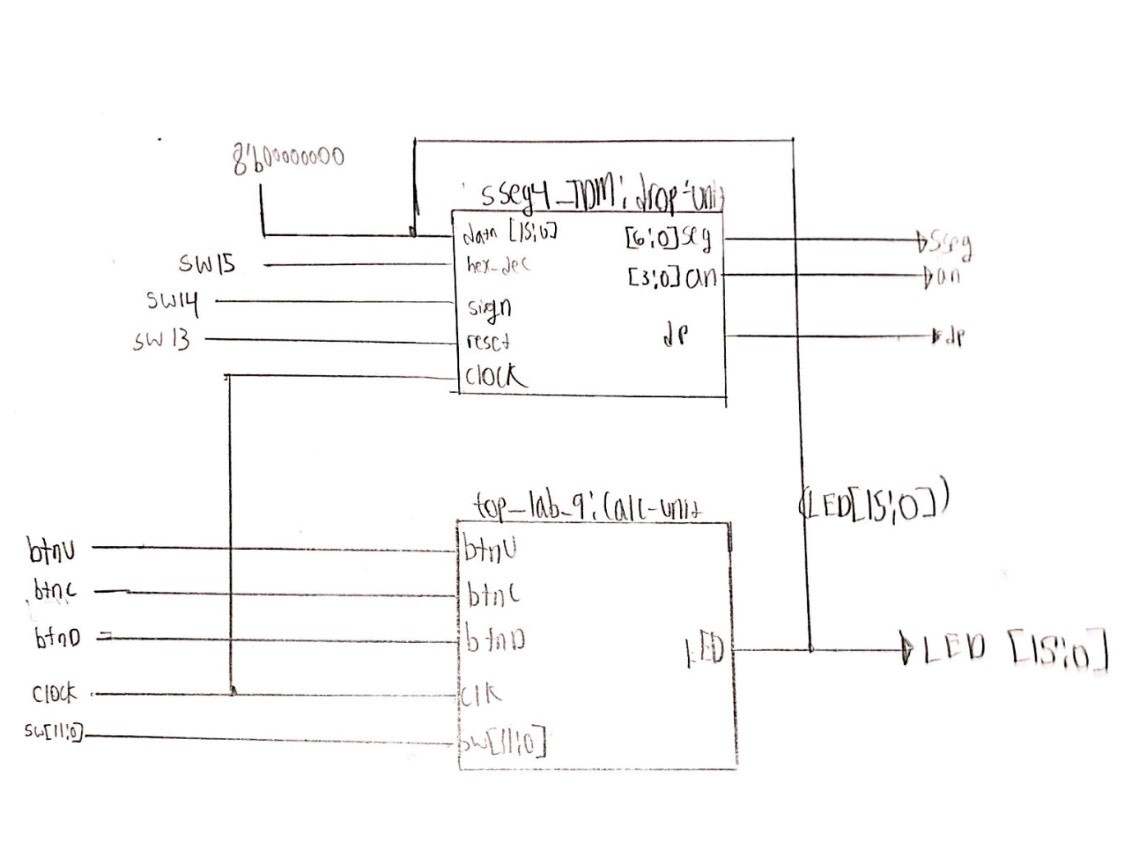
\includegraphics[width=1.0\textwidth]{Calculator}
	\caption{Figure 10.3 with boxes}
	\label{fig:sim_with_table}=
\end{figure}
\clearpage
\begin{figure}[ht]\centering
	
	\includegraphics[width=1.0\textwidth]{sseg4_tdm}
	\caption{Figure 10.3 with boxes}
	\label{fig:sim_with_table}=
\end{figure}
\clearpage





\section*{Code}


\begin{lstlisting}[style=Verilog,caption=Counter Code ,label=code:ex ]

// Chris Jones , ELC 2137, 2020 -3-30-20

module counter #(parameter N=1) 
(
input clk, rst, en,
output [N-1:0] count , 
output tick
);
// internal signals
reg [N-1:0] Q_reg , Q_next;
// register (state memory)
always @(posedge clk, posedge rst)
begin
if (rst)
Q_reg <= 0;
else 
Q_reg <= Q_next;
end
// next -state logic
always @*
begin
if (en)
Q_next = Q_reg + 1;
else
Q_next = Q_reg; // no change 
end
// output logic 
assign count = Q_reg; 
assign tick = (Q_reg=={N{1'b1}}) ? 1'b1 : 1'b0;

endmodule


\end{lstlisting}



\begin{lstlisting}[style=Verilog,caption= Counter Test Bench,label=code:ex ]

// Chris Jones , ELC 2137, 2020 -3-30-20

module counter_test();

reg clk, en, rst;
wire [1:0} count;
wire tick;

counter #(.N(2)) a(.clk(clk), .en(en), .rst(rst),
.count(count), .tick(tick));

always begin 
clk = ~clk;
#5;
end

initial begin 
clk = 0; en = 1; rst = 1; #5;
clk = 1; en = 1; rst = 1; #5;
clk = 0; en = 1; rst = 1; #5;
clk = 1; en = 1; rst = 1; #5;
clk = 0; en = 1; rst = 1; #5;
clk = 1; en = 1; rst = 1; #5;
clk = 0; en = 1; rst = 1; #5;
clk = 1; en = 1; rst = 1; #5;
clk = 0; en = 1; rst = 1; #5;
clk = 1; en = 1; rst = 1; #5;
clk = 0; en = 0; rst = 0; #5;
clk = 1; en = 0; rst = 0; #5;
clk = 0; en = 0; rst = 0; #5;
clk = 1; en = 0; rst = 0; #5;
clk = 0; en = 0; rst = 0; #5;
clk = 1; en = 0; rst = 0; #5;
clk = 0; en = 0; rst = 0; #5;
clk = 1; en = 0; rst = 0; #5;
clk = 0; en = 0; rst = 0; #5;
clk = 1; en = 0; rst = 0; #5;
clk = 0; en = 1; rst = 0; #5;
clk = 1; en = 1; rst = 0; #5;
clk = 0; en = 1; rst = 0; #5;
clk = 1; en = 1; rst = 0; #5;
clk = 0; en = 1; rst = 0; #5;
clk = 1; en = 1; rst = 0; #5;
clk = 0; en = 1; rst = 0; #5;
clk = 0; en = 1; rst = 0; #5;
clk = 1; en = 1; rst = 0; #5;
clk = 0; en = 1; rst = 0; #5;
$finish;
end


\end{lstlisting}


\begin{lstlisting}[style=Verilog,caption= sseg4 TDM code ,label=code:ex ]
// Chris Jones , ELC 2137, 2020 -3-30-20

module sseg4_TDM(
input [15:0] data,
input hex_dec, sign,
input reset,
input clock,
output [6:0] seg, 
output dp,
output[3:0] an
);

wire [15:0] ebout, mux2out;
wire [3:0] mux4out;
wire [6:0] decout;
wire andecout;
wire m2sel;
wire [1:0] digit_sel;
wire tickout;

counter #(.N(18)) c1(.clk(clock), .rst(reset), .en(1), .tick(tickout));
counter #(.N(18)) c2(.clk(clock), .on(tickout), .count(digit_sel), .rst(reset));
BCD11 e0(.in(data[10:0]), .out(ebout));
mux2 #(.N(16)) mux2A(.in0(data), .in1(ebout), .sel(hex_dec), .out(mux2out));
mux4 #(.N(4)) mux4A(.in0(mux2out[3:0]), .in1(mux2out[7:4]), .in2(mux2out[11:8]), .in3(mux2out[15:12]), .sel(digit_sel), .out(mux4out));
sseg_decoder s1(.num(mux4out), .sseg(decout));
an_decoder an1(.in(digit_sel), .out(an));
assign m2sel = ~an[3];
and agate1(andecout, sign, m2sel);
mux2 #(.N(7)) mux2B(.in0(decout), .in1(7'b01111111), .sel(andecout), .out(seg));
assign dp = 1;
endmodule

\end{lstlisting}


\begin{lstlisting}[style=Verilog,caption= sseg4 TDM test bench code ,label=code:ex ]
// Chris Jones , ELC 2137, 2020 -3-30-20

module  sseg_TDM_test();

reg [15:0] data;
reg hex_dec;
reg sign;
reg reset;
reg clock;
wire [6:0] seg;
wire [3:0] an;
wire dp;

sseg4_TDM st(.data(data), .hex_dec(hex_dec), .sign(sign), .reset(reset), .clok(clock), .seg(seg), .an(an), .dp(dp));

always begin
clock = ~clock; #5;
end

initial begin
clock = 0;
data = 16'b0000000000000010;
hex_dec = 0;
sign = 0;
reset = 0;
#20;
data = 16'b0000000000000001;
hex_dec=1;
sign = 0;
reset = 0;
#40;
data = 16'b0000000000000010;
hex_dec=0;
sign= 0;
reset = 0;
#80;
data = 16'b0000000000000010;
hex_dec = 1;
sign = 0;
reset = 0;
#160
data = 16'b0000000000000011;
hex_dec = 0;
sign = 0;
reset = 1;
#160;
data = 16'b0000000000000011;
hex_dec= 1;
sign = 0;
reset = 0;
#320;
data = 16'b0000000000000100;
hex_dec = 0;
sign = 0;
reset = 0;
#640;
data = 16'b0000000000000100;
hex_dec = 1;
sign = 0;
reset = 0;
#1280;
data= 16'b0000000000000101;
hex_dec = 0;
sign = 0;
reset = 0;
#2560;
data = 16'b0000000000000101;
hex_dec = 1;
sign = 0;
reset = 0;
#5120;
data = 16'b0000000000000110;
hex_dec = 0;
sign = 0;
reset = 0;
#10240
data = 16'b0000000000000110;
hex_dec = 1;
sign = 0;
reset = 0;
#20480;
data = 16'b0000000000000111;
hex_dec = 0;
reset = 0;
#40960;
$finish;
end
endmodule
	

\end{lstlisting}




\end{document}

